\documentclass[a4paper,11pt]{article}
\usepackage[utf8]{inputenc}
\usepackage{textcomp}
\usepackage{lmodern}
\usepackage{listings}
\usepackage{graphicx}
\usepackage{listings}
\usepackage{color}
\usepackage{url}
\usepackage{verbatim}
\usepackage[top=3cm,bottom=3cm,left=3cm,right=3cm]{geometry}

\title{Master in Cyber-Security\\
	LINGI2146 --- Mobile and Embedded Computing: \\
	Publishing IoT Sensor Data through a MQTT publish/subscribe infrastructure}

\author{FONTAINE Romain, NYAKI Loïc, TIO NOGUERAS Gérard}

\begin{document}
\maketitle
\newpage
\tableofcontents

\newpage

\section{Introduction}
When using sensors to measure data, such as light, temperature or noise, it is common to use a IoT device : a small battery-powered piece of hardware, equipped with one or several sensors, that can communicate data wirelessly.\\

The way to propagate information is by communicating with neighbouring devices, which will forward the information towards a specific device, called a root node. To be able to communicate in this manner, each device must form a relationship with the other nodes and form what is called a Wireless Mesh Network (WMN).\\

Another part of this system is the MQTT infrastructure. MQTT (Message Queuing Telemetry Transport) is a publish/subscribe messaging protocol that allows publishers to publish data to a MQTT broker, while clients can subscribe to that same broker, to receive specific information from the publishers.\\

The first goal of this project is to implement a custom routing protocol, similar to RPL,  that will allow the creation of a network of IoT devices. Information should be able to go from any node of the network, to the root node, which acts as a gateway towards the outside world. \\

The second goal is to create an MQTT infrastructure, that can allow clients to subscribe to a MQTT broker, and publishers to publish data to the broker.\\

The third and last goal is then to create a gateway agent that will serve as an interface between the IoT network and the MQTT infrastructure, in such a way that the IoT devices should be able to become MQTT publishers, and any client from outside the IoT network should be able to subscribe to the MQTT broker, and be periodically updated with data from the IoT network sensors.

\begin{comment}
First, we need implement a custom routing protocol for sensor networks, similar to RPL, on top of 6LoWPAN which is a special version of IPv6 for low-power devices. Then, we build a messaging infrastructure using MQTT, which is a publish/subscribe messaging protocol. Lastly, we interface the sensor network with the MQTT message infrastructure, by using a border router, whose job will be to translate the message travelling between the sensor network and the MQTT message infrastructure.
\\
Lastly, the sensor data 
\end{comment}
\section{System Architecture}
The scope of this project covers 

\begin{figure}
  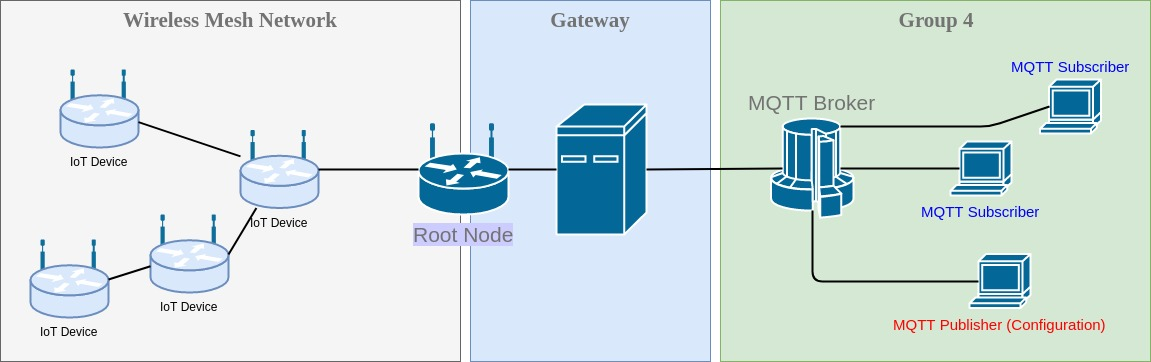
\includegraphics[width=\linewidth]{img/network-diagram-1.jpg}
  \caption{An overview of the system.}
  \label{fig:network1}
\end{figure}
\section{DODAG and Routing Protocol}
One of the objectives of this project is the implementation of a routing protocol, similar to RPL (Routing Protocol for Low-Power and Lossy Networks). A routing protocol is needed in order create a Destination Oriented Directed Acyclic Graph (DODAG), and have the information propagate properly from any individual node to the root node of the network.\\

Any given node that isn't part of the network should have a way to become a member of the network, and start publishing information. Any node of the network should also be able to disappear without compromising the integrity of the network as long as the node is not a critical junction of two parts of the network graph.

\subsection{Joining a graph}
When an IoT device is started, it needs to find a network to join. It will therefore broadcast a message asking around for some information about the graph, and wait for the response. This message will be send periodically.\\

When a node that is already part

\subsection{Leaving a graph}

\subsection{Routing Message Types}
\subsubsection{Routing Message Format}


\section{MQTT infrastructure}
MQTT stands for Message Queuing Telemetry Transport, and is a publish/subscribe protocol. It requires a MQTT broker as well as MQTT clients that can publish information to the broker, as topics, or subscribe to the broker for a specific topic, in order to be given the required information through time.

\subsection{MQTT Broker}
The broker is the central element of MQTT. It is where each MQTT client either subscribe to a topic, or publishes information under a specific topic. In this instance, we used Mosquitto, an open-source MQTT broker.

\subsection{MQTT Publishers}
\subsection{MQTT Subscribers}

\section{Rime-MQTT Gateway}
\subsection{Wireless Mesh Network Configuration}

\end{document}

